\begin{table*}[h]
\renewcommand{\arraystretch}{1.2}
\begin{subtable}{0.22\textwidth}
\centering
\begin{tabular}{c}
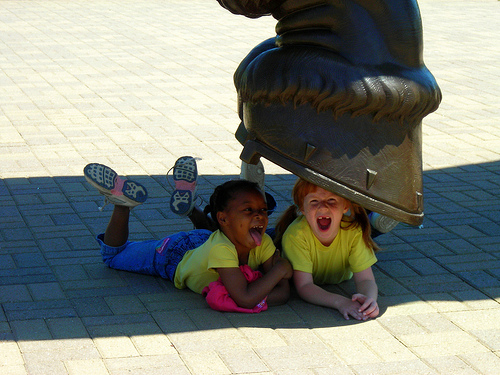
\includegraphics[width=0.7\textwidth]{chapters/IJCNLP/images/533602654.jpg}
\end{tabular}
\end{subtable}%
\begin{subtable}{0.75\textwidth}
\begin{tabular}{rp{27em}}
Source: & two children on their stomachs lay on the ground under a pipe \\
NMT: & zwei kinder \textcolor{red}{auf ihren gesichtern} liegen unter dem boden auf dem boden \\
Ours: & zwei kinder liegen bäuchlings auf dem boden unter einer \textcolor{red}{schaukel}
 \\
\end{tabular}
\end{subtable}

\vspace{0em}

\begin{subtable}{0.22\textwidth}
\centering
\begin{tabular}{c}
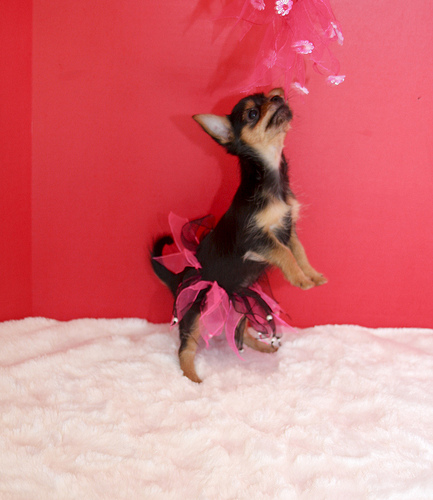
\includegraphics[width=0.7\textwidth]{chapters/IJCNLP/images/3720366614.jpg}
\end{tabular}
\end{subtable}%
\begin{subtable}{0.75\textwidth}
\begin{tabular}{rp{27em}}
Source: & small dog in costume stands on hind legs to reach dangling flowers \\
NMT: & ein kleiner hund steht auf dem hinterbeinen und \textcolor{red}{läuft} , \textcolor{red}{nach links von blumen zu sehen}  \\
Ours: & ein kleiner hund in einem kostüm steht auf den hinterbeinen , um die blumen zu erreichen\\
\end{tabular}

\end{subtable}

\vspace{0em}

\begin{subtable}{0.22\textwidth}
\centering
\begin{tabular}{c}
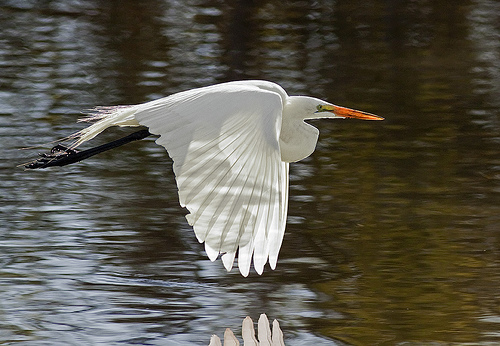
\includegraphics[width=0.7\textwidth]{chapters/IJCNLP/images/3325578605.jpg}
\end{tabular}
\end{subtable}%
\begin{subtable}{0.75\textwidth}
\begin{tabular}{rp{27em}}
Source: & a bird flies across the water \\
NMT: & ein vogel fliegt über das wasser \\
Ours: & ein vogel fliegt \textcolor{red}{durch} das wasser\\
\end{tabular}
\end{subtable}

\caption{Examples where our model improves or worsens the translation compared to the NMT baseline. Top: NMT translates the wrong body part; both models skip ``pipe''. Middle: NMT incorrectly translates the verb and misses several nouns. Bottom: Our model incorrectly translates the preposition.}\label{tab:results:examples}
\end{table*}
